\documentclass[11pt,a4paper]{article}

\usepackage[utf8]{inputenc}
\usepackage[T1]{fontenc}
\usepackage[spanish,es-noshorthands]{babel}
\usepackage{mathptmx}
\usepackage{amsmath,amssymb}
\usepackage{graphicx}
\usepackage{booktabs}
\usepackage{tabularx}
\usepackage{array}
\usepackage{geometry}
\usepackage{float}
\usepackage{caption}
\usepackage{enumitem}
\usepackage{xcolor}
\usepackage[hidelinks]{hyperref}

\geometry{margin=2.5cm}
\captionsetup{font=small,labelfont=bf}
\setlist[itemize]{topsep=2pt,itemsep=2pt,parsep=0pt}
\setlist[enumerate]{topsep=2pt,itemsep=2pt,parsep=0pt}

\title{Comparación de decodificación con modelos ocultos de Markov en un caso didáctico de riesgo de incendio forestal: anteproyecto reproducible}

\author{
Oscar Alonso De la Pava Suarez\\
Anderson Jesus Ospina Cardona\\
Kevin Andrés Valencia Daza\\[0.4em]
\small Grupo de trabajo 11\\
\small Ingeniería de Software y Datos, IUDigital\\
\small Curso de Simulación\\
\small Docente asesor: Julián Andrés Loaiza López
}

\date{9 de noviembre de 2026}

\begin{document}

\maketitle

\begin{center}
\textbf{Etiqueta del entregable:} anteproyecto\\
\textbf{Versión:} manuscrito de anteproyecto con resultados D4 y referencias verificadas\\
\textbf{Declaración de uso de IA:} aprobada por el grupo de trabajo 11 el 2026-11-09
\end{center}

\begin{abstract}
\noindent
Este anteproyecto estudia, con fines exclusivamente didácticos, si la estructura temporal de un modelo oculto de Markov (HMM) aporta alguna ventaja frente a reglas simples de humedad en un caso de riesgo de incendio forestal sin datos de campo. Los estados latentes \(s_1\), \(s_2\) y \(s_3\) se tratan como etiquetas puras; la humedad se representa de forma ordinal como Alta, Media o Baja, sin porcentajes ni umbrales físicos inventados. Se fijaron las matrices \(A\), \(B\) y \(\pi\) del material del caso y se compararon tres reglas de decisión con parámetros ``oráculo'': M0, un umbral determinista sobre la humedad actual; M1, un baseline con la ley observable exacta y prior estacionario de \(A\); y M2, el HMM completo con \(A\), \(B\) y \(\pi\). El diseño fue pareado, con \(T=500\) pasos por secuencia, \(N=2000\) secuencias sintéticas, una semilla distinta por secuencia y agregación de métricas por secuencia mediante media, desviación estándar e intervalo de confianza del 95\,\% por bootstrap.

En el escenario base, la macro-F1 fue 0.6608 para M0, 0.6749 para M1 y 0.6749 para M2. En el escenario con \(B\) alterada, la macro-F1 descendió a 0.4912, 0.4966 y 0.4965, respectivamente. M1 y M2 resultaron prácticamente indistinguibles; además, M0 conservó un mayor recall de \(s_3\) en ambos escenarios. Estas cifras son simuladas y no permiten afirmar validez ecológica, capacidad predictiva sobre incendios reales ni superioridad general del HMM. El aporte del anteproyecto es el protocolo reproducible, el código y la comparación controlada, no una conclusión aplicada.

\vspace{0.5em}
\noindent\textbf{Palabras clave:} modelos ocultos de Markov, decodificación, Viterbi, Forward--Backward, macro-F1, simulación, reproducibilidad.
\end{abstract}

% ------------------------------------------------------------------
\section{Introducción}

\subsection{Planteamiento del problema y justificación}

El material del caso describe un entorno forestal en el que se registran niveles ordinales de humedad ---Alta, Media y Baja--- y se plantea explorar si un HMM permite inferir estados supuestos de riesgo: Riesgo Bajo, Riesgo Moderado y Riesgo Extremo. No se aporta un conjunto de datos sensorizados reales y se advierte que la humedad por sí sola no demuestra el nivel de riesgo en el terreno. Por tanto, el problema es didáctico y computacional: formalizar un HMM, distinguir la inferencia de estados latentes del entrenamiento de parámetros y evaluar de forma controlada distintas reglas de decodificación.

La justificación del ejercicio es metodológica. Un HMM puede parecer atractivo porque incorpora persistencia temporal, pero esa ventaja no debe presuponerse. Si no se compara contra alternativas simples y no se reporta incertidumbre, el uso del modelo puede confundirse con una preferencia técnica. Este anteproyecto adopta la opción honesta: los estados son regímenes latentes asociados a humedad y la palabra ``riesgo'' funciona como etiqueta didáctica, no como una variable física medida.

\subsection{Preguntas de investigación}

\begin{itemize}
  \item \textbf{P1.} ¿Cómo formalizar un HMM de tres estados y tres observaciones ordinales de humedad sin introducir umbrales físicos ni datos no disponibles?
  \item \textbf{P2.} Con \(A\), \(B\) y \(\pi\) fijos, ¿cómo se comparan M0, M1 y M2 en macro-F1, recall de \(s_3\) y exactitud sobre secuencias sintéticas pareadas?
  \item \textbf{P3.} ¿Cómo cambia esa comparación cuando se altera la matriz de emisión \(B\) para reducir la separabilidad entre estados?
\end{itemize}

\subsection{Objetivos y aportes}

\textbf{Objetivo general:} formular, implementar y evaluar de forma reproducible una comparación de decodificación con un HMM didáctico de tres estados, sin afirmar validez ecológica.

\textbf{Objetivos específicos:}
\begin{enumerate}
  \item Formalizar el HMM con estados \(s_1\), \(s_2\), \(s_3\), observaciones ordinales Alta/Media/Baja y parámetros \(A\), \(B\) y \(\pi\) fijos.
  \item Implementar y comparar M0, M1 y M2 en un diseño pareado con \(T=500\) y \(N=2000\), reportando macro-F1, recall de \(s_3\) y exactitud por secuencia.
  \item Evaluar un escenario secundario con \(B\) alterada y documentar sus límites.
\end{enumerate}

\textbf{Aportes del anteproyecto:}
\begin{itemize}
  \item Un protocolo explícito con parámetros, semillas, métricas y criterios de agregación.
  \item Código reproducible con pruebas automatizadas y artefactos trazables.
  \item Una comparación que separa la estructura del modelo de la calidad de estimación, porque los tres modelos reciben parámetros ``oráculo''.
  \item Una lista explícita de limitaciones y pendientes, sin inventar hallazgos ni referencias.
\end{itemize}

% ------------------------------------------------------------------
\section{Estado del arte (provisional)}

Los HMM son un marco clásico para procesos con estados latentes y observaciones indirectas. Los trabajos fundacionales de Rabiner \cite{rabiner1989} y Baum et al. \cite{baum1970} sistematizaron los problemas de evaluación, decodificación y aprendizaje. La literatura aplicada es amplia en voz, bioinformática, diagnóstico industrial y análisis de series temporales. Sin embargo, este anteproyecto \textbf{no realizó todavía una revisión sistemática}; por tanto, no se presenta una síntesis crítica cerrada ni se usan referencias no verificadas.

El vacío que motiva este ejercicio no es un vacío de la literatura, sino una necesidad docente: mostrar cómo se distingue la inferencia con parámetros conocidos del entrenamiento, cómo se evita la fuga de información y cómo se reporta la incertidumbre. La comparación con M0 y M1 es deliberadamente conservadora: si el HMM no supera baselines simples en un escenario didáctico, no hay razón para atribuirle una ventaja aplicada.

\textbf{Pendiente:} protocolo de búsqueda, bases consultadas, criterios de inclusión, deduplicación y síntesis crítica. Las referencias incluidas ya fueron verificadas por el equipo; la revisión sistemática de literatura sigue pendiente.

% ------------------------------------------------------------------
\section{Marco teórico}

\subsection{Definición del HMM}

Un HMM discreto se especifica mediante \(\lambda=(S,V,A,B,\pi)\), donde:
\begin{itemize}
  \item \(S=\{s_1,s_2,s_3\}\) es el conjunto de estados latentes, tratados como etiquetas puras.
  \item \(V=\{\text{Alta},\text{Media},\text{Baja}\}\) es el alfabeto ordinal de observaciones de humedad.
  \item \(A=[a_{ij}]\) es la matriz de transición, con \(a_{ij}=P(S_t=s_j\mid S_{t-1}=s_i)\) y filas que suman 1.
  \item \(B=[b_i(k)]\) es la matriz de emisión, con \(b_i(k)=P(O_t=v_k\mid S_t=s_i)\) y filas que suman 1.
  \item \(\pi=[\pi_i]\) es la distribución inicial en \(t=1\), con \(\pi_i=P(S_1=s_i)\) y suma 1.
\end{itemize}

Las matrices usadas son las del material del caso:
\begin{equation}
A=
\begin{bmatrix}
0.70 & 0.25 & 0.05\\
0.30 & 0.50 & 0.20\\
0.10 & 0.30 & 0.60
\end{bmatrix},
\qquad
B=
\begin{bmatrix}
0.70 & 0.25 & 0.05\\
0.20 & 0.60 & 0.20\\
0.05 & 0.25 & 0.70
\end{bmatrix},
\qquad
\pi=[0.50,\;0.30,\;0.20].
\end{equation}

\subsection{Supuestos y decisiones de interpretación}

\begin{itemize}
  \item \textbf{Estados como etiquetas puras (D3.1):} \(s_1\), \(s_2\) y \(s_3\) no tienen una definición física. ``Riesgo Bajo'', ``Riesgo Moderado'' y ``Riesgo Extremo'' son alias mnemónicos.
  \item \textbf{Humedad ordinal (D3.2):} Alta \(>\) Media \(>\) Baja. No se usan porcentajes ni umbrales numéricos.
  \item \textbf{Paso de observación (D3.3):} un paso es una ocasión de observación, sin unidad física. ``Día'' solo se usa como convención editorial.
  \item \textbf{\(\pi\) como prior inicial (D3.5):} \(\pi\) no es la distribución estacionaria de \(A\). La estacionaria calculada es aproximadamente \([0.424,0.348,0.227]\), distinta de \(\pi\).
  \item \textbf{Persistencia:} la duración media en cada estado es aproximadamente 3.3, 2.0 y 2.5 pasos.
  \item \textbf{Supuesto de \(B\):} más humedad se asocia a menos riesgo en la matriz del material. Es un supuesto didáctico, no evidencia de campo.
\end{itemize}

\subsection{Los tres problemas clásicos y el alcance de este anteproyecto}

\begin{enumerate}
  \item \textbf{Evaluación:} calcular \(P(O_{1:T}\mid\lambda)\) con Forward.
  \item \textbf{Decodificación:} obtener la ruta más probable con Viterbi o las posteriores marginales con Forward--Backward.
  \item \textbf{Aprendizaje:} estimar \(A\), \(B\) y \(\pi\) con Baum--Welch.
\end{enumerate}

Este anteproyecto se limita a \textbf{D5a: inferencia con \(A\), \(B\) y \(\pi\) fijos}. Implementa Forward, Forward--Backward y Viterbi. \textbf{No implementa Baum--Welch}; el entrenamiento queda fuera del núcleo y solo podría añadirse como anexo D5b con partición por secuencia, inicializaciones múltiples, alineación de estados y control de convergencia.

\subsection{Modelos comparados}

\begin{itemize}
  \item \textbf{M0 --- umbral determinista:} asigna a cada observación el estado con mayor probabilidad en \(B\). Con las matrices del caso: Alta \(\rightarrow s_1\), Media \(\rightarrow s_2\), Baja \(\rightarrow s_3\). Solo usa la humedad actual.
  \item \textbf{M1 --- baseline observable con prior estacionario:} usa \(A\), \(B\) y la distribución estacionaria \(\xi\) de \(A\) en lugar de \(\pi\). La ley observable exacta se deriva como \(p_O=\xi B\) y \(Q=P(S\mid O)^{\top}(AB)\). Esta es la forma no degenerada de explotar la estructura observable sin usar las etiquetas latentes. En este caso el mapeo M0 es biyectivo, por lo que M1 y M2 comparten \(A\) y \(B\) y difieren en el prior inicial.
  \item \textbf{M2 --- HMM completo:} usa \(A\), \(B\) y \(\pi\). La regla primaria es el argmax de la posterior marginal de Forward--Backward; Viterbi queda disponible como análisis de sensibilidad.
\end{itemize}

\subsection{Métricas}

\begin{itemize}
  \item \textbf{Macro-F1:} promedio no ponderado del F1 de las tres clases. Es la métrica principal porque no deja que la clase mayoritaria domine el resultado.
  \item \textbf{Recall de \(s_3\):} proporción de pasos con estado verdadero \(s_3\) que fueron identificados como \(s_3\). Es secundaria y relevante porque \(s_3\) es la clase extrema.
  \item \textbf{Exactitud:} proporción de pasos correctamente clasificados. Es secundaria y puede ocultar desbalances.
\end{itemize}

Las métricas se calculan por secuencia y luego se agregan. La unidad independiente es la secuencia, no el paso de tiempo.

% ------------------------------------------------------------------
\section{Metodología}

\subsection{Diseño experimental}

\begin{itemize}
  \item \textbf{Diseño pareado:} las tres variantes reciben exactamente las mismas observaciones y se comparan contra los mismos estados latentes.
  \item \textbf{Tamaño:} \(T=500\) pasos por secuencia; \(N=2000\) secuencias.
  \item \textbf{Semillas:} una semilla maestra (\texttt{20261109}) y una semilla distinta por secuencia, derivada y registrada. No se reinicia la misma semilla en réplicas supuestamente independientes.
  \item \textbf{Agregación:} media, desviación estándar e intervalo de confianza del 95\,\% por bootstrap de secuencias (1000 réplicas).
  \item \textbf{Escenarios:} base y \(B\) alterada. Ambos comparten \(T\), \(N\), semilla maestra y regla de decisión.
\end{itemize}

\subsection{Generación de datos}

Para cada secuencia se simulan estados latentes a partir de \(\pi\) y \(A\), y observaciones a partir de \(B\). No se usan datos reales ni se ajustan parámetros con las etiquetas verdaderas. Los estados verdaderos se usan solo para evaluar, nunca para elegir el modelo ni para inicializar M1 o M2.

\subsection{Reglas de decisión}

\begin{itemize}
  \item \textbf{M0:} \(\hat{s}_t=\arg\max_i B_{i,O_t}\).
  \item \textbf{M1:} HMM con \(A\), \(B\) y \(\xi\); \(\hat{s}_t=\arg\max_i P(S_t=s_i\mid O_{1:T})\).
  \item \textbf{M2:} HMM con \(A\), \(B\) y \(\pi\); misma regla de posterior marginal. La ruta de Viterbi se conserva como sensibilidad.
\end{itemize}

\subsection{Escenario con \(B\) alterada}

La \(B\) alterada se construye mezclando cada fila de \(B\) con la distribución uniforme:
\begin{equation}
B_{\text{alt}}=(1-m)B+m\,\mathbf{1}/3,
\end{equation}
con \(m=0.5\) \textbf{provisional}. Al aumentar \(m\), las emisiones se vuelven menos separables y el problema de decodificación se dificulta. El valor de \(m\) no está aprobado como decisión científica y debe fijarse antes de reportar el escenario como definitivo.

\subsection{Reproducibilidad}

La ejecución completa se realizó con:
\begin{verbatim}
python main.py --save outputs/protocolo_d4_resumen.json
\end{verbatim}

Los artefactos son:
\begin{itemize}
  \item \texttt{outputs/protocolo\_d4\_resumen.json}: resumen estructurado, semillas y matrices.
  \item \texttt{outputs/protocolo\_d4\_resumen.csv}: tabla larga con media, desviación e IC.
  \item \texttt{outputs/protocolo\_d4\_resumen.md}: tablas legibles.
  \item \texttt{outputs/protocolo\_d4\_metricas.png}: figura de métricas.
  \item \texttt{outputs/protocolo\_d4\_ejecucion.log}: salida de consola.
\end{itemize}

Las tablas y la figura se regeneran con \texttt{python scripts/report\_d4.py}. Las pruebas se ejecutan con \texttt{python -m pytest -q}.

\subsection{Fases metodológicas}

\begin{table}[H]
\centering
\caption{Fases metodológicas y evidencia.}
\begin{tabularx}{\textwidth}{@{}l>{\raggedright\arraybackslash}X>{\raggedright\arraybackslash}X@{}}
\toprule
Fase & Actividad & Evidencia\\
\midrule
F1 & Protocolo y alcance & \texttt{decisiones.md}, D1--D6\\
F2 & Materiales del caso & \texttt{materiales/caso\_riesgo\_de\_incendio\_forestal.md}\\
F3 & Formalización del HMM & \texttt{src/hmm\_model.py}; sección 3\\
F4 & Implementación y pruebas & \texttt{src/simulation.py}; \texttt{tests/test\_protocol.py}\\
F5 & Simulación pareada & \texttt{outputs/protocolo\_d4\_resumen.json}\\
F6 & Métricas e intervalos & \texttt{outputs/protocolo\_d4\_resumen.csv}\\
F7 & Manuscrito de anteproyecto & este documento\\
\bottomrule
\end{tabularx}
\end{table}

% ------------------------------------------------------------------
\section{Resultados}

Todas las cifras provienen de la ejecución del 2026-11-09 con \(T=500\), \(N=2000\) y semilla maestra 20261109. Son \textbf{simuladas}. Los intervalos son IC 95\,\% por bootstrap de secuencias.

\subsection{Escenario base}

\begin{table}[H]
\centering
\caption{Escenario base. Media e IC 95\,\% por bootstrap de secuencias.}
\begin{tabular}{lccc}
\toprule
Modelo & Macro-F1 (media [IC 95\,\%]) & Recall \(s_3\) & Exactitud\\
\midrule
M0 & 0.6608 [0.6599, 0.6618] & 0.6996 [0.6976, 0.7015] & 0.6650 [0.6641, 0.6660]\\
M1 & 0.6749 [0.6738, 0.6760] & 0.6691 [0.6667, 0.6714] & 0.6828 [0.6817, 0.6838]\\
M2 & 0.6749 [0.6738, 0.6759] & 0.6691 [0.6666, 0.6715] & 0.6828 [0.6818, 0.6839]\\
\bottomrule
\end{tabular}
\end{table}

\subsection{Escenario con \(B\) alterada}

\begin{table}[H]
\centering
\caption{Escenario con \(B\) alterada. Media e IC 95\,\% por bootstrap de secuencias.}
\begin{tabular}{lccc}
\toprule
Modelo & Macro-F1 (media [IC 95\,\%]) & Recall \(s_3\) & Exactitud\\
\midrule
M0 & 0.4912 [0.4902, 0.4922] & 0.5163 [0.5142, 0.5184] & 0.4991 [0.4982, 0.5001]\\
M1 & 0.4966 [0.4953, 0.4979] & 0.3999 [0.3970, 0.4029] & 0.5236 [0.5223, 0.5248]\\
M2 & 0.4965 [0.4952, 0.4977] & 0.3996 [0.3968, 0.4025] & 0.5236 [0.5224, 0.5248]\\
\bottomrule
\end{tabular}
\end{table}

\subsection{Figura de métricas}

\begin{figure}[H]
\centering
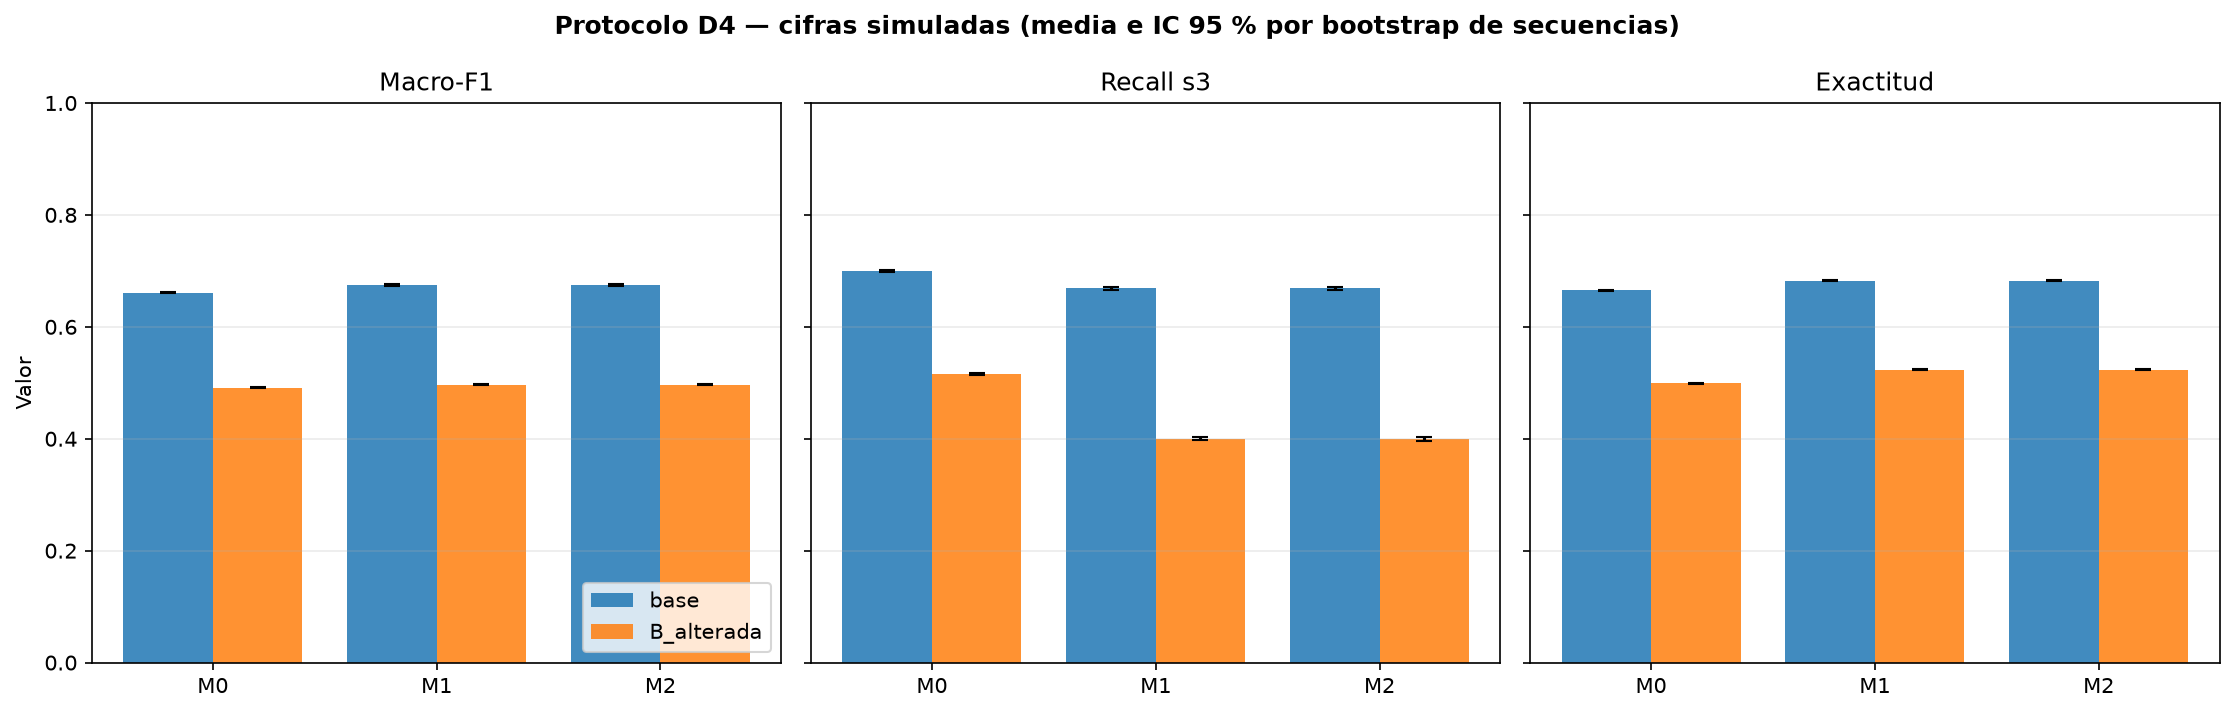
\includegraphics[width=\textwidth]{outputs/protocolo_d4_metricas.png}
\caption{Macro-F1, recall de \(s_3\) y exactitud por modelo, con IC 95\,\% por bootstrap de secuencias. Cifras simuladas.}
\label{fig:metricas}
\end{figure}

\subsection{Observaciones descriptivas}

\begin{itemize}
  \item En el escenario base, M1 y M2 superan a M0 en macro-F1 y exactitud, pero M0 tiene mayor recall de \(s_3\).
  \item M1 y M2 son prácticamente indistinguibles: en el escenario base coinciden hasta la cuarta cifra decimal; con \(B\) alterada difieren en menos de \(7\times10^{-5}\) en macro-F1. Esto es consistente con que solo cambia el prior inicial y \(T\) es largo.
  \item Con \(B\) alterada, las tres variantes caen de forma marcada. M1 y M2 mejoran apenas la macro-F1 y la exactitud de M0, pero pierden aproximadamente 12 puntos porcentuales de recall de \(s_3\).
  \item No se realizaron pruebas de hipótesis formales. Los IC son descriptivos y no deben interpretarse como una prueba de superioridad.
\end{itemize}

% ------------------------------------------------------------------
\section{Discusión}

El resultado central es sobrio: en este caso didáctico, la estructura temporal del HMM mejora la macro-F1 y la exactitud frente al umbral determinista, pero no mejora el recall de la clase extrema. Además, M1 y M2 producen resultados casi idénticos, lo que sugiere que, con \(T=500\), el efecto del prior inicial es despreciable frente al efecto de \(A\) y \(B\). Esto no demuestra que el HMM sea superior; muestra que la comparación depende de la métrica y del escenario.

La diferencia entre M1 y M2 es pequeña por construcción: ambos usan \(A\) y \(B\), y solo difieren en \(\pi\) frente a la estacionaria \(\xi\). Si se quisiera una línea base más exigente, habría que definir otra forma de M1; sin embargo, esa modificación no se hizo en este anteproyecto y queda como decisión pendiente para un trabajo futuro. La \(B\) alterada reduce la separabilidad de las emisiones y hace que las tres variantes se acerquen; al mismo tiempo, M1 y M2 pierden recall de \(s_3\). Es un recordatorio de que una mejora agregada puede ocultar un deterioro en la clase de mayor interés.

El alcance es limitado. Los estados son etiquetas puras, la humedad es ordinal, los parámetros son hipotéticos y los datos son simulados. No se contrasta con literatura porque la revisión sistemática está pendiente. Tampoco se afirma que estos resultados se generalicen a incendios reales.

% ------------------------------------------------------------------
\section{Conclusiones}

\textbf{Respuesta a P1.} El HMM puede formalizarse de manera completa con \(S=\{s_1,s_2,s_3\}\), \(V=\{\text{Alta},\text{Media},\text{Baja}\}\), \(A\), \(B\) y \(\pi\), sin inventar porcentajes de humedad ni definiciones físicas para los estados. La formalización es suficiente para implementar Forward, Forward--Backward y Viterbi.

\textbf{Respuesta a P2.} Con \(A\), \(B\) y \(\pi\) fijos, en el escenario base M1 y M2 obtuvieron macro-F1 \(\approx 0.6749\) y exactitud \(\approx 0.6828\), frente a 0.6608 y 0.6650 de M0. Sin embargo, M0 obtuvo mayor recall de \(s_3\) (0.6996 frente a 0.6691). La conclusión depende de la métrica y no autoriza a afirmar superioridad general.

\textbf{Respuesta a P3.} Con \(B\) alterada, las tres variantes cayeron a macro-F1 \(\approx 0.49\). M1 y M2 apenas superaron a M0 en macro-F1 y exactitud, pero perdieron recall de \(s_3\). El escenario es sensible a la matriz de emisión y su valor de mezcla sigue siendo provisional.

\textbf{Trabajo futuro:} activar D5b con Baum--Welch y partición por secuencia; definir una M1 alternativa si el equipo lo considera necesario; fijar el valor de \(B\) alterada; añadir pruebas de hipótesis y tamaños de efecto; completar la revisión de literatura; y, solo si se obtienen datos adecuados, explorar una validación externa.

% ------------------------------------------------------------------
\section{Limitaciones}

\begin{itemize}
  \item Los resultados son simulados y no tienen validez ecológica.
  \item Los estados \(s_1\), \(s_2\), \(s_3\) son etiquetas puras; ``riesgo'' es un alias didáctico.
  \item La humedad es ordinal; no se usan porcentajes ni umbrales físicos.
  \item Los parámetros \(A\), \(B\) y \(\pi\) son hipotéticos y fijos; no se estimaron de datos reales.
  \item M1 y M2 comparten \(A\) y \(B\); la comparación no aísla una línea base completamente distinta.
  \item La \(B\) alterada usa una mezcla provisional de 0.5 con la uniforme.
  \item No se realizaron pruebas de hipótesis formales; los IC son descriptivos.
  \item La revisión sistemática de literatura sigue pendiente; las referencias incluidas fueron verificadas por el equipo.
  \item El manuscrito se entrega en Markdown y en LaTeX; la compilación local queda pendiente porque el entorno de trabajo no tiene TeX instalado.
\end{itemize}

% ------------------------------------------------------------------
\section{Declaración de uso de IA}

Se utilizó un asistente de programación basado en IA (OpenCode) para apoyar la organización del protocolo, la implementación del código, la generación de tablas y la redacción del manuscrito. Las decisiones científicas registradas en \texttt{decisiones.md} fueron expresadas por el grupo de trabajo 11. Las cifras reportadas provienen de código ejecutado y son simuladas. \textbf{Declaración aprobada por el grupo de trabajo 11 el 2026-11-09.}

% ------------------------------------------------------------------
\begin{thebibliography}{9}

\bibitem{rabiner1989}
L. R. Rabiner, ``A tutorial on hidden Markov models and selected applications in speech recognition,'' \emph{Proceedings of the IEEE}, vol. 77, no. 2, pp. 257--286, 1989.

\bibitem{baum1970}
L. E. Baum, T. Petrie, G. Soules y N. Weiss, ``A maximization technique occurring in the statistical analysis of probabilistic functions of Markov chains,'' \emph{The Annals of Mathematical Statistics}, vol. 41, no. 1, pp. 164--171, 1970.

\bibitem{caso}
Caso didáctico ``Evaluación de riesgo de incendio forestal,'' \texttt{materiales/caso\_riesgo\_de\_incendio\_forestal.md}. Documento interno, no publicado.

\bibitem{plantilla}
Plantilla de artículo Q1 proporcionada en el curso, \texttt{materiales/plantilla\_articulo.pdf}. Documento interno, no publicado.

\end{thebibliography}

% ------------------------------------------------------------------
\appendix

\section{Reproducibilidad}

\begin{verbatim}
# Entorno
python -m venv .venv
.\.venv\Scripts\Activate.ps1
pip install -r requirements.txt

# Pruebas
python -m pytest -q

# Ejecución completa D4
python main.py --save outputs/protocolo_d4_resumen.json

# Tablas y figura
python scripts/report_d4.py --input outputs/protocolo_d4_resumen.json
\end{verbatim}

Estructura relevante:
\begin{itemize}
  \item \texttt{main.py}: ejecutor del protocolo.
  \item \texttt{src/hmm\_model.py}: HMM, Forward, Forward--Backward y Viterbi.
  \item \texttt{src/simulation.py}: M0/M1/M2, métricas y experimento D4.
  \item \texttt{tests/test\_protocol.py}: pruebas del protocolo.
  \item \texttt{scripts/report\_d4.py}: tablas y figura desde el JSON.
  \item \texttt{outputs/}: resultados simulados.
  \item \texttt{legacy/}: simulación exploratoria anterior.
  \item \texttt{decisiones.md}: bitácora D1--D6.
\end{itemize}

\section{Trazabilidad de decisiones}

\begin{table}[H]
\centering
\caption{Trazabilidad de las decisiones registradas.}
\begin{tabularx}{\textwidth}{@{}l>{\raggedright\arraybackslash}X>{\raggedright\arraybackslash}X@{}}
\toprule
ID & Decisión & Evidencia\\
\midrule
D1 & Ejercicio didáctico, sin validez ecológica & \texttt{decisiones.md}\\
D2 & Escenarios hipotéticos; toda cifra se rotula como simulada & \texttt{decisiones.md}\\
D3.1--D3.5 & Estados como etiquetas puras; humedad ordinal; paso de observación; constructo honesto; \(K=3\) y \(\pi\) inicial & \texttt{decisiones.md}\\
D4 & M0/M1/M2, macro-F1 principal, recall \(s_3\) y exactitud secundarias; \(T=500\); \(N=2000\); \(B\) alterada & \texttt{decisiones.md}; \texttt{outputs/protocolo\_d4\_resumen.json}\\
D5 & D5a: solo decodificación con \(A\), \(B\) y \(\pi\) fijos & \texttt{decisiones.md}; \texttt{src/hmm\_model.py}\\
D6 & Aprobador/revisor grupo 11; alcance; etiqueta anteproyecto; legado aislado & \texttt{decisiones.md}; \texttt{legacy/}\\
\bottomrule
\end{tabularx}
\end{table}

\end{document}
